% Graph paper
% Based on: http://www.texample.net/tikz/examples/graph-paper
\documentclass{article}
%\usepackage{nopageno}
\usepackage{geometry}
\geometry{hmargin=1.5cm,vmargin=1.42cm, voffset=-2mm}
\usepackage{tikz}
\def\width{17.5cm}
\def\hauteur{25cm}

\begin{document}

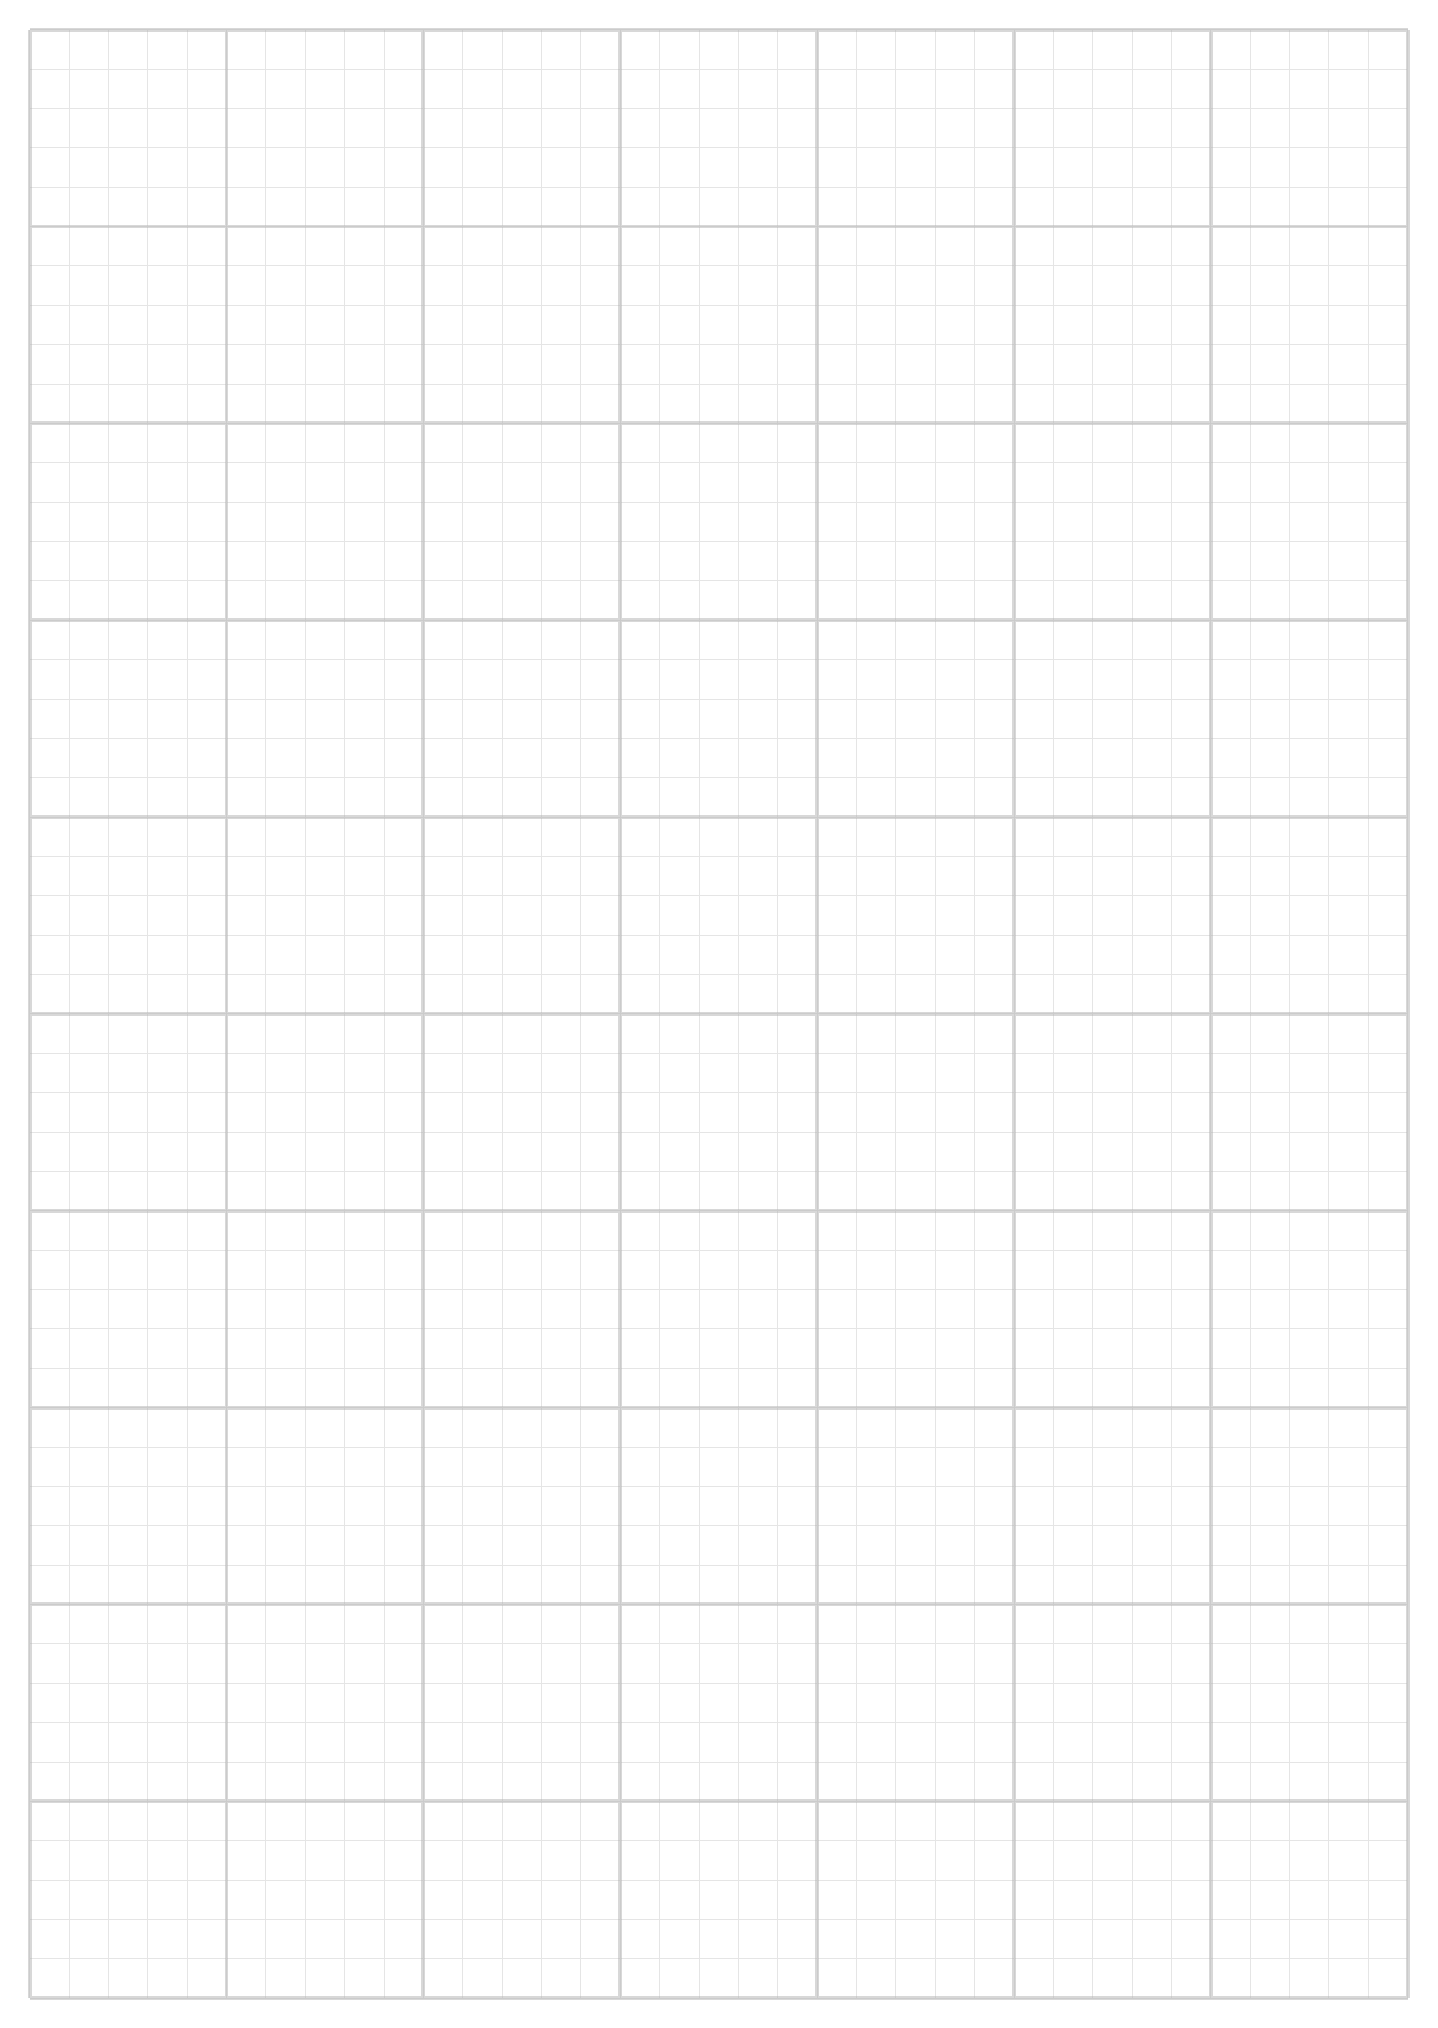
\begin{tikzpicture}[x=1cm, y=1cm, semitransparent]
    \draw[step=0.5cm, line width=0.1mm, black!20!white] (0,0) grid (\width,\hauteur);
%\draw[step=5cm, line width=0.2mm, black!40!white] (0,0) grid (\width,\hauteur);
    \draw[step=2.5cm, line width=0.5mm, black!30!white] (0,0) grid (\width,\hauteur);
%\draw[step=1cm, line width=0.3mm, black!90!white] (0,0) grid (\width,\hauteur);
\end{tikzpicture}


\end{document}
